\chapter{Configuração}\label{cha:configuration}\label{conf:configuration}
O XCSoar é um computador de planeio altamente configurável e pode ser personalizado para se adequar a uma grande variedade de preferências e necessidades do usuário.  A configuração toda é salva em um arquivo de perfil, que abriga todos os ajustes.  Sempre que uma configuração for valiosa, é aconselhável ter uma cópia de segurança do arquivo do perfil (veja seção \ref{sec:profiles}. Este capítulo descreve os ajustes de configurações e opções)..

\section{Escopo da configuração}

Há várias maneiras para se personalizar o XCSoar:
\begin{itemize}

\item Modificando os ajustes das configurações.  Esta lista de configurações é, preferencialmente, feita pelos usuários e foi dada atenção especial para isto neste documento.
\item Alterando o idioma ou mesmo mudando as palavras do texto na interface do usuário.
\item Alterando os botões e suas funções.  Permite que se mude o conteúdo e estrutura dos botões dos menus.
\item Alterando ou adicionando ações desempenhadas quando alguns eventos do computador de planeio são feitos.
\item Definindo quanto tempo uma mensagem de estado aparece e fica audível e quando estas mensagens irão ocorrer.
\end{itemize}
%Describing all of these in a detail level like a reference manual would 
%do is beyond the scope of this document. The user is referred to browse 
%through the XCSoar Wiki for more details. 
%\url{http://www.xcsoar.org/trac/wiki}

\section{Modificando ajustes}

Existe um enorme conjunto de ajustes das configurações que podem ser personalizados pelas janelas, acessíveis pelo menu:
\begin{jspecs}
\item[\bmenug{Config 2/3}\blink\bmenug{Sistema}] ativa a janela de configuração principal para vários ajustes estáticos.  Não é permitido que seja acessado durante o vôo.
\item[\bmenug{Config 2/3}\blink\bmenug{Planador}] Janela para especificar os dados do planador, com a polar e a carga alar sendo os mais importantes.  Esta janela deverá ser inclusa na verificação antes do vôo se a base do XCSoar é usada em diferentes aeronaves.
\item[\bmenug{Config 2/3}\blink\bmenug{Dispositivos}] configuração dos dispositivos conectados ao XCSoar.  Também sendo uma janela de ajuste do sistema, em raros casos, será necessária antes da decolagem.  Quando as conexões com os dispositivos forem perdidas, esta janela deve ser usada para reconecta-los.  Esta janela não foi e não será usada para o vôo.  Infelizmente, podem ocorrer problemas com o hardware e criar esta demanda ocasionalmente.  
\end{jspecs}

\section{Configure o sistema}
A configuração do sistema pode ser acessada através de um menu de duas camadas 
\marginlabel{\bmenug{Config 2/3}\blink\bmenug{Sistema}}
ou sequencialmente através dos botões frente/trás.

\begin{center}
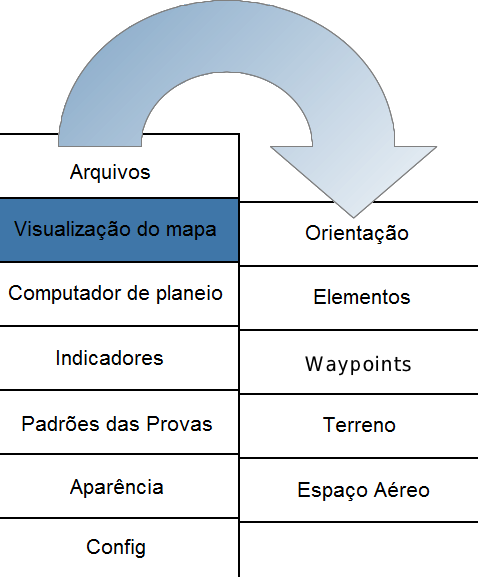
\includegraphics[angle=0,width=0.5\linewidth,keepaspectratio='true']{figures/config-menu.png}
\end{center}

Você deve ser fortemente desencorajado para fazer alterações durante o vôo.  Todas as mudanças das configurações devem ser feitas no solo para que os efeitos desejados no comportamento do programa possam ser verificados.

A janela de ajustes também contém diversas páginas.  Uma vez feitas alterações, clique em FECHAR ou PWR/ESC no Altair para fechar a janela e retornar ao menu de configuração.  Qualquer outra tecla retorna ao modo normal de mapa.

\tip Se estiver contente com os ajustes das configurações, salve o arquivo de perfil e faça uma cópia de segurança, caso tenha que restaurar os ajustes se a memória do seu PDA for acidentalmente apagada.

Veja o capítulo ~\ref{cha:data-files} para descrição do formato de arquivos relativos aos ajustes.  Se não for usado nenhum arquivo, o campo pode deixar em branco.  Os campos no formulário de nome do arquivo mostram os arquivos que correspondem ao filtro de extensão de arquivos.  Isto torna mais fácil achar e selecionar o arquivo correto.

A janela de configuração principal (Ajuste do sistema) pode rodar em nível Básico ou Avançado através de um campo no canto superior esquerdo da janela.  
\sketch{figures/config-expert.png}
Quando está no modo Básico, alguns ajustes menos usados (ou mais avançados) são ocultados.  Nas descrições abaixo, todos os parâmetros marcados com asterisco estão visíveis somente no modo avançado.

%%%%%%%%%%%%%%%%%%
\section{Arquivos / Arquivos}
A janela especifica os arquivos mais importantes que devem ser configurados quando se voa em um local novo.

\begin{description}
\item[Caminho dos dados do XCSoar]  a localização de todos os seus dados do XCSoar no seu disco rígido, cartão SD ou memória estática do PDA.
\item[Base de dados do Mapa]  o nome do arquivo de mapa contento elevação digital, dados do terreno, topografia e opcionalmente, waypoints, espaço aéreo, etc.  Um bom arquivo de banco de dados cobre todas as necessidades para esta página.
\item[Waypoints]  arquivo primário de waypoint.  Se deixado em branco, os waypoints serão carregados do mapa (se houverem).
\item[Mais waypoints*]  arquivo secundário de waypoints.  Deve ser usado para adicionar waypoints para competições.
\item[Waypoints observados*]  arquivo de waypoints contendo waypoints especiais para os quais os podem substituir os cálculos adicionais de altura de chegada no mapa.  Útil para waypoints como fontes de térmicas conhecidas (ex, usinas) ou passagens por montanhas.
\item[Espaço aéreo]  arquivo de espaço aéreo primário.  Se deixado em branco, os espaços aéreos serão carregados do arquivo de mapa (se disponíveis).
\item[Mais espaços aéreos*] arquivo secundário de espaço aéreo.
\item[Detalhes de Waypoint] o aeródromo pode conter suplementos de rotas ou outras informações sobre aeródromos individuais
\end{description}

Os arquivos de espaço aéreo definem o Uso Especial do Espaço Aéreo (Special Use Airspace – SUA).  Até dois arquivos podem ser usados, o primeiro para o arquivo principal de SUA e o segundo por exemplo, para usar com espaço aéreo NOTAM.
\sketch{figures/config-site.png}

O conceito da base de dados do mapa do XCM é para ajustar um local para voar.  As versões do XCSoar antes da v6.4 necessitavam que cada arquivo fosse separado e especificados separadamente (como ‘arquivo de terreno’ e ‘arquivo de topografia’, respectivamente.  Esta opção foi descartada pelo banco de dados do mapa XCM com o lançamento do XCSoar versão 6.4.

O arquivo de mapa XCM contém todos estes três arquivos: terreno, topografia e opcionalmente waypoints e espaço aéreos.  Se o último contiver por exemplo o arquivo primário de waypoint, deve ser deixado em branco e o sistema irá carregar os waypoints do arquivo do mapa.  Porém, o usuário pode especificar outros arquivos e estes serão usados ao invés dos dados do arquivo de mapa.

Veja Seção~\ref{sec:map} para mais detalhes sobre o arquivo de mapas.  


%%%%%%%%%%%%%%%%%%
\section{Visualização do Mapa / Orientação}\label{sec:map-projection}

Esta página permite você especificar a orientação preferida do mapa e visualização.

\begin{description}
\item[Orientação Cruzeiro/Girando]  \label{conf:orientation} determina como a tela é rotacionada com o planador, dependendo do modo de visualização da tela.  \\
  {\bf Rota acima}: a exibição do mapa será rotacionada para que a rota do planador seja orientada para cima.  A seta de símbolo de norte aponta para o norte verdadeiro.  O símbolo da aeronave pode ser mostrado rotacionando de acordo com a direção computada da aeronave, levando em consideração o vento. \\
  \sketch{figures/config-map_projection.png}
  {\bf Heading up}: a exibição do mapa será rotacionada e a aeronave é orientada para cima. \\
  {\bf Norte acima}: a exibição do mapa será sempre orientada de norte a sul e o ícone da aeronave será rotacionando para mostrar seu trajeto (corrigido pelo vento). \\
  {\bf Alvo acima}: a exibição do mapa será rotacionada para que o alvo atual seja orientado para cima. \\
  {\bf Wind up} :  a exibição do mapa será rotacionando para que o vento sempre seja orientado acima-abaixo (talvez útil para se voar onda).
\item[Zoom Girando]  \label{conf:circlingzoom} determina os níveis de zoom que deverão ser mantidos para modo girando e cruzeiro.  Se ativo, o zoom aumentará automaticamente quando entrar em modo de giro e diminuirá quando deixar este modo.
\item[Referência de mudança de mapa]  a direção de acordo com o mapa será mostrada para que apresente uma seção do mapa legível. \\
  {\bf Nenhum}: Todos os ajustes desativados. \\
  {\bf Rota}: use uma média recente da trilha no chão como base. \\
  {\bf Alvo}: Use o waypoint atual como base.
\item[Compensação de posição do planador]  \label{conf:gliderposition} define a localização da aeronave desenhada na tela em percentual da borda da tela.
\item[Distância máxima de auto zoom]  Limite superior para a distância de auto zoom.
\end{description}


%%%%%%%%%%%%%%%%%%
\section{Visualização do Mapa / Elementos}\label{sec:map-elements}

Esta página fornece opções relativas aos elementos da tela sobrepostos à exibição do mapa.

\begin{description}
\item[Rastro no chão]  mostra o rastro no chão (projeção) no mapa.  O ajuste ‘Auto” mostra o rastro se somente houver diferença significante para a direção da aeronave.
\item[Tráfego FLARM]  \label{conf:flarm-on-map} ativa a exibição do tráfego FLARM no mapa.
\item[Comprimento da trilha*] \label{conf:snailtrail} determina o tamanho da trilha desenhada atrás do planador. \\
\sketch{figures/config-map_elements.png}
  {\bf Desligado}: nenhuma trilha é desenhada. \\
  {\bf Longo}: é desenhada trilha longa (aprox. 60 minutos). \\
  {\bf Curto}: É desenha trilha curta (aprox. 10 minutos). \\
  {\bf Completo}: desenhada a trilha para o vôo todo.
\item[Deriva da trilha*] \label{conf:traildrift} determina quando a trilha é derivada com o vento quando mostrado em modo girando.  Desligado, a trilha permanece sem compensação de deriva.
\item[Tipo de rastro*] \label{conf:snailtype} ajusta o tipo de exibição da trilha. \\
  {\bf Vario \#1}: dentro de áreas de ascensão, a linha é verde e fina, na descendente a linha é marrom e fina.  Vôo reto, a linha é cinza. \\
  {\bf Vario \#1 (com pontos)}: o mesmo padrão do anterior, mas com linhas pontilhas enquanto afunda. \\
  {\bf Vario \#2}: na subida a linha vai de laranja para vermelha, no afundamento é mostrada de azul claro para azul escuro.  Vôo reto é amarela. \\
  {\bf Vario \#2 (com pontos)}: mesmo do padrão anterior, mas com linhas pontilhadas enquanto afunda. \\
  {\bf Altitude}:as cores correspondem à altitude.
\item[Rastro escalonado*] \label{conf:trailscaled} se ajustado para ‘Ligado’ a trilha será escalonada de acordo com o sinal do variômetro.
\item[Marcadores de custo de desvio*]  se ativado, no modo cruzeiro exibe alguns números projetados na frente do nariz do planador.  É a distância adicional em porcentagem que se você voar na posição da figura e após voar reto para o alvo, comparado à distância reta para o alvo.
\item[Símbolo da aeronave*]  Ajuste o símbolo de sua aeronave. \\
  {\bf Simples}: gráfico de linhas simples com um planador negro com contornos brancos. \\
  {\bf Simples (largo)}: aumenta o gráfico ‘Simples’ para melhor visibilidade. \\
  {\bf Detalhado}: mostra o planador com detalhes. \\
  {\bf HangGlider}: asa-delta simples branca com contornos negros. \\
  {\bf ParaGlider}: SParaglider simples branco com contornos negros.
\item[Seta de vento*]  determina a forma que a seta de vento é desenhada no mapa. \\
  {\bf Desligado}: não será desenhada seta. \\
  {\bf Ponta de seta}: desenha somente a ponta da seta. \\
  {\bf Seta completa}: desenha uma seta com a cabeça com linha pontilhada.  Áreas de triânguloFAI: mostra triângulos FAI no mapa.
\item[Áreas de triângulo FAI] Mostra as áreas de triângulos FAI no mapa.
  
\end{description}


%%%%%%%%%%%%%%%%%%
\section{Visualização do Mapa / Waypoints}\label{sec:waypoint-display}

Esta página mostra as opções relativas à exibição do mapa.

\begin{description}
\item[Formato do rótulo]  este ajuste  \label{conf:labels} determina o rótulo mostrado 
  para cada waypoint, com cinco opções diferentes: \\
  {\bf Nome completo}: o nome completo de cada waypoint é mostrado. \\
  {\bf Primeira palavra do nome}: somente a primeira palavra (até o primeiro espaço) do nome do waypoint é mostrada.
\sketch{figures/config-map_waypoint.png} \\
  {\bf Primeiras 3 letras}: as primeiras 3 letras do nome do waypoint são mostradas. \\
  {\bf Primeiras 5 letras}: primeiras 5 letras do nome do waypoint são mostradas. \\
  {\bf Nenhum}: nenhum nome do waypoint é mostrado.
\item[Altura de chegada*] \label{conf:arrivalheight} ativa a informação mostrada da altura de chegada para locais pousáveis. \\
  {\bf Nenhum}: Não é mostrada altura de chegada. \\
  {\bf Planeio direto}: altura de chegada com planeio direto (não é considerada a topografia do terreno). \\
  {\bf Planeio evitando terreno}:altura de chegada considerando evitar possíveis obstáculos do terreno.  \\
  {\bf Direto \& Terreno}: ambas alturas de chegada serão mostradas. \\
  {\bf Taxa de planeio requerida}: mostra a taxa de planeio sobre o solo necessária para alcançar o waypoint.
\item[Estilo de rótulo*]  podem ser mostrados os rótulos para pousáveis por um retângulo com fundo branco ou com linhas pontilhadas.
\item[Visibilidade do rótulo*]  \label{conf:labelvisibility} controla quais waypoints serão mostrados com nomes e altitudes de chegada no mapa: \\
  {\bf Tudo}: All waypoint labels will be displayed. \\
  {\bf Task waypoints \& airfields}: todos os waypoints da prova e aeródromos serão mostrados. \\
  {\bf Waypoints da prova \& pousáveis}:todos os waypoints da prova e pousáveis serão mostrados.
  {\bf Waypoints da prova:}: todos os waypoints da prova serão mostrados. \\
  {\bf Nenhum}:  nenhum waypoint da prova será mostrado.
\item[Símbolo pousáveis]  \label{conf:waypointicons} três símbolos estão disponíveis: círculo roxo, com alto contraste com os ícones e ícones com luz de tráfego. Veja seção~\ref{sec:waypoint-schemes} para detalhes.
\item[Detalhar pousáveis*]  ativa os detalhes dos pousáveis ao invés de ícones fixos, com informações diversas sobre o comprimento da pista e direção.
\item[Tamanho pousável*]  é mostrada uma porcentagem do tamanho selecionado dos pousáveis.
\item[Escala comprimento pista*]  ativando esta opção irá exibir para os pousáveis detalhados, o comprimento real da pista de pouso.
\end{description}


%%%%%%%%%%%%%%%%%%
\section{Visualização do Mapa / Terreno}\label{sec:terrain-display}

Esta página ajusta como o terreno e topologia são desenhados no mapa. 
\sketch{figures/config-terrain.png}
O efeito da alteração dos ajustes do terreno é visto abaixo:

\begin{description}
\item[Exibição terreno]  mostra a elevação digital do terreno no mapa.
\item[Exibir topografia]  mostra as características topográficas do mapa (estradas, rios, lagos, etc).
\item[Cores do terreno]  define as cores usadas na renderização.  Vários tons estão disponíveis que funcionam melhor para você dependendo do relevo de sua região (montanhas, planícies, planaltos, etc).
\item[Sombreamento*]  \label{conf:shading} o terreno pode ser sombreado ao longo de encostas para indicar tanto a direção do vento quando a posição solar ou sombreamento fixo norte-leste.  As encostas com face para o vento (ou sol) são exibidas mais brilhantes e as encostas com face oposta ao vento ficam escurecidas.
\item[Contraste do terreno*]  define a quantidade de sombra no terreno.  Use valores altos para enfatizar as encostas, valores baixos se voar em montanhas altas.  
\item[Brilho terreno*]  define o brilho da renderização do terreno.  Este item controla a iluminação do terreno.
\item[Contornos] ativa/desativa os contornos do terreno. 
\end{description}


As cores dos terrenos são ilustradas na tabela abaixo:

\begin{longtable}{c c c c}
\em{Planícies [m]} & \em{Montanhas [m]} & \em{ICAO [m]} & \em{Cinza [m]} \\
\nopagebreak[4]
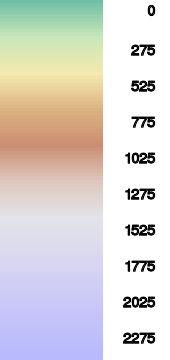
\includegraphics[angle=0,width=3.0cm,keepaspectratio='true']{figures/ramp-terrain-flatlands.png}&
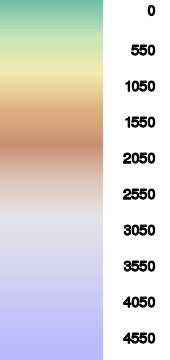
\includegraphics[angle=0,width=3.0cm,keepaspectratio='true']{figures/ramp-terrain-mountanous.png}&
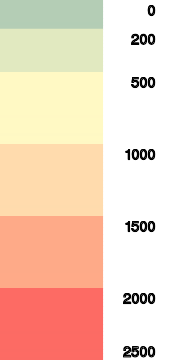
\includegraphics[angle=0,width=3.0cm,keepaspectratio='true']{figures/ramp-terrain-icao.png}&
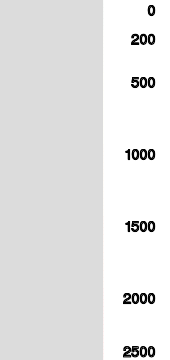
\includegraphics[angle=0,width=3.0cm,keepaspectratio='true']{figures/ramp-terrain-grey.png}
\end{longtable}

\begin{longtable}{c c c c}
\em{Imhof 4 [m]} & \em{Imhof 7 [m]} & \em{Imhof 12 [m]} & \em{Imhof Atlas [m]} \\
\nopagebreak[4]
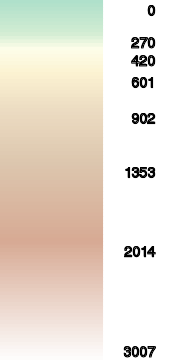
\includegraphics[angle=0,width=3.0cm,keepaspectratio='true']{figures/ramp-terrain-imhof4.png}&
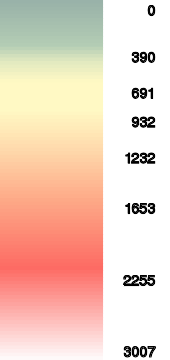
\includegraphics[angle=0,width=3.0cm,keepaspectratio='true']{figures/ramp-terrain-imhof7.png}&
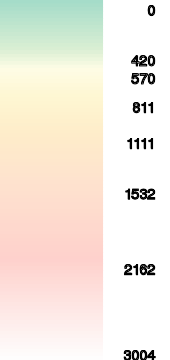
\includegraphics[angle=0,width=3.0cm,keepaspectratio='true']{figures/ramp-terrain-imhof12.png}&
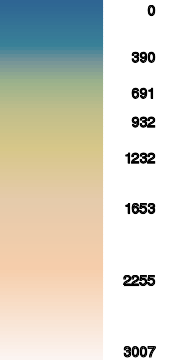
\includegraphics[angle=0,width=3.0cm,keepaspectratio='true']{figures/ramp-terrain-imhofatlas.png}
\end{longtable}


%%%%%%%%%%%%%%%%%%
\section{Visualização do Mapa / Espaço Aéreo }

Esta página é usada para determinar como a informação do espaço aéreo é mostrada e como os alertas são emitidos.

\begin{description}
\item[Exib Espaço Aéreo]  Ccontrola como são filtrados os alertas e espaços aéreos baseados na altitude.  A janela de filtro de espaço aéreo também permite filtrar a exibição e alertas independente para cada classe de espaço aéreo. \\
  {\bf Todos ligados}: todas as informações de espaço aéreo são mostradas ao mesmo tempo. \\
  {\bf Cortar}: somente espaço aéreo acima de uma altitude determinado pelo usuário será mostrado. \\
  {\bf Auto}: somente espaço aéreo na altitude atual, com margem de tolerância definida pelo usuário (+/-).
\sketch{figures/config-airspace.png} \\
  {\bf Todos abaixo}:  como o modo Auto adicionando os espaços aéreos abaixo da aeronave.
\item[Avisos] determina se os alertas estarão ativos ou inativos.
\item[Tempo do aviso*]  tempo estimado antes da invasão que o sistema irá avisar o piloto.
\item[Tempo de reconhecimento*]  este é o período que um alerta de espaço aéreo foi reconhecido e não será repetido.
\item[Usar outline preto*]  desenha uma linha externa ao redor de cada espaço aéreo.
\item[Modo de preenchimento do espaço aéreo*]  especifica o modo de preenchimento da área do espaço aéreo. \\
  {\bf Preencher tudo}:  preenche com transparência as cores de espaço aéreo de todas as áreas. \\
  {\bf Preenchimento}: desenha uma linha sólida com a metade da borda transparente ao redor do espaço aéreo. \\
  {\bf Padrão}:  esta seleção é a melhor opção para o seu hardware.
  {\bf No Fill}: não há preenchimento.
\end{description}

Esta página também contém botões  \button{Cores} e \button{Filtro} que podem ser usados para visualizar ou alterar as cores/padrões usados para cada classe de espaço aéreo e quando cada espaço aéreo poderá ser filtrado de alertas e/ou exibição.  Dependendo do ajuste da transparência do espaço aéreo não é necessário definir padrões.  A disponibilidade da transparência recai na capacidade do hardware e pode haver diferenças.

\subsection*{Cores}
Esta função é usada para determinar as cores para cada classe de espaço aéreo.  Primeiro selecione o espaço aéreo que deseja alterar e selecione a cor e padrão que deseja para a classe do espaço aéreo.

\subsection*{Filtros}
A função do filtro é descrita na Seção~\ref{sec:airspace-filter}.


%%%%%%%%%%%%%%%%%%
\section{Computador de Planeio / Fatores de Segurança}

Esta página permite definir as alturas de segurança e comportamentos para os pousos alternativos.

\begin{description}
\item[Altura de chegada]  a altura acima do terreno que o planador deverá chegar para pousar com segurança.
\item[Altura do terreno]  \label{conf:safetyterrain} altura acima do terreno que o planador deve planar no planeio final.  Veja seção
  ~\ref{sec:safety-heights} para mais detalhes dos significados de altura de segurança. \\
\item[Modo alternativo]  \label{conf:alternatesmode} determina o tipo de pousos alternativos conforme abaixo: \\
  {\bf Simples}: os alternativos irão ser ordenados pela altura de chegada.  O primeiro waypoint na lista é o que está mais ao alcance.   \\
  {\bf Prova}: a ordem irá levar em conta a direção da prova atual mostrará de acordo com a distância mínima extra navegada ao respeito campo e adiante na prova. \\
  {\bf Casa}: a ordem tentará achar opções de pouso na direção atual do ponto configurado como casa.  Semelhante ao ‘Prova’, mas com o ponto Casa como destino.
\item[Degradação da polar*]  degradação permanente da polar. 0 significa sem degradação.  50 indica que o afundamento da aeronave foi dobrado.\label{conf:safetyMC} 
\item[Fator de Risco STF*] 
 o fator de risco STF reduz o ajuste de MacCready usado para calcular a velocidade ideal quando o planador está baixo para compensar o risco.  Ajuste 0,0 para não compensado, 1,0 faz o 
\sketch{figures/config-safety.png}
 MacCready linear com o peso (com referência à altura de subida máxima).  Se optar por esta configuração, o valor de 0,3 pode ser recomendado.  Veja Seção ~\ref{sec:safety-para} mais detalhes.
\end{description}


%%%%%%%%%%%%%%%%%%
\section{Computador de Planeio / Computador de Planeio}\label{sec:final-glide}\label{conf:final-glide}	

Esta página permite configurar os algoritmos do computador de planeio.

\begin{description}
\item[Modo Auto MC]  esta opção define qual algoritmo de MacCready automático será usado. Para mais detalhes, veja a seção ~\ref{sec:auto-maccready}. \\
  {\bf Planeio final}: ajuste de MacCready para chegada mais rápida no planeio final.
\sketch{figures/config-glidecomputer.png} \\
  {\bf Tendência média de subida}: ajuste do MacCready para a tendência média de subida baseada em todas as subidas. \\
  {\bf Ambos}: Usa a tendência média durante a prova e a chegada rápida quando em planeio final.
\item[Bloquear Speed to fly*]  se ativo, o comando velocidade de cruzeiro é ajustada para a velocidade ideal MacCready sem movimento vertical de massa de ar.  Se inativo, o comando velocidade de cruzeiro é ajustado para a velocidade ideal golfinho, equivalente à velocidade MacCready com movimento vertical de massa de ar.
\item[Nav. por altitude baro*]  quando ativo e se conectado a um altímetro barométrico, a altitude barométrica é usada para todas as funções de navegações.  Caso contrário, a altitude GPS será usada.
\item[Flap força cruzeiro*]
 quando ativo, faz os interruptores dos flaps no Vega a forçarem o modo de cruzeiro quando o flap não está positivo. Significa que, quando sai de uma termal, alternar para flap neutro ou negativo irá imediatamente alternar o modo do XCSoar para modo de cruzeiro.  Igualmente, para o sistema Borgelt B50, o comando de velocidade força o XCSoar a alternar para modo de subida ou cruzeiro.
\item[GR Average period*]  eficiência média é sempre calculada em tempo real.  Neste campo você pode decidir em quantos segundos de vôo este cálculo deve ser feito.  A distância real coberta segundo a segundo neste período é dividida pela distância final ou altitude.  Se, por exemplo, você for e retornar ao mesmo ponto depois de 2 minutos e você tem um ajuste de 2 minutos como período, a média da taxa de planeio irá considerar a distância total coberta nestes dois minutos e não a distância de sua posição 2 minutos atrás e sua posição atual, que neste caso pode ser quase zero!  Normalmente para planadores, um valor razoável é de 90 a 120 segundos e para paragliders, 15 segundos.  Valores baixos irão fornecer resultados muito semelhantes à taxa de planeio instantânea (GR Inst) e valores altos irão se assemelhar a taxa de planeio em cruzeiro (GR Cruize).  Outros instrumentos comerciais e softwares usam 2 minutos.
\item[Deriva do vento prevista*]  \label{conf:predict-drift}cálculo para deriva do vento com a duração prevista do modo girando.  Isto reduz a altura de chegada com vento de nariz (padrão).
\end{description}


%%%%%%%%%%%%%%%%%%
\section{Computador de Planeio / Vento} \label{sec:wind}

Esta página configura a base de cálculo para o vento.

\begin{description}
\item[Vento aut]  \label{conf:autowind} permite ativar/desativar o algoritmo de vento automático. \\
  {\bf Manual}: o algoritmo é desligado e o piloto é responsável pelo ajuste de estimativa de vento. \\
  {\bf Girando}: este modo necessita somente de uma fonte de GPS. \\
  {\bf ZigZag}: necessita de um variômetro inteligente com saída para velocidade do vento. \\
  {\bf Ambos}:  Usa  Girando e ZigZag.
\item[Prefere external wind]  se ativo, o vetor de vento recebido pelos dispositivos externos se sobrepõe ao cálculo interno de vento do XCSoar.
\end{description}


%%%%%%%%%%%%%%%%%%
\section{Computador de Planeio / Rota}

Esta página permite controlar os cálculos de planeio e otimizações de rota.

\begin{description}
\item[Modo rota]  \label{conf:routemode} quais tipos de obstáculos são usados no planejamento da rota.  Veja a seção ~\ref{sec:route} 
para as descrições detalhadas.
\item[Modo de chegada]  \label{conf:turningreach} como os cálculos são feitos para o alcance do planeio respeitando o terreno. \\
  {\bf Desligado}: cálculos de alcance desligado. \\
  {\bf Direto}: o alcance é uma linha reta. \\
  {\bf Virando}: o alcance é calculado permitindo curvas ao redor dos obstáculos do terreno.
\item[Polar de chegada*]  \label{conf:reachpolar} determina o desempenho do planeio usado no alcance nos cálculos de chegada de pousável, aborto e alternativos. \\
  {\bf Prova}: usa o valor de MacCready da prova. \\
  {\bf MC de Segurança}: usa o valor de MacCready de segurança.
\end{description}

%%%%%%%%%%%%%%%%%%
\section{Indicadores / FLARM, Outro} \label{sec:flarmandother-gauge}

\begin{description}
\item[FLARM radar]  \label{conf:flarmdisplay} ativa a exibição do mostrador do radar FLARM.  A direção da trilha do alvo relativo à trilha da aeronave é mostrada como uma ponta de seta e um triângulo apontando para cima ou para baixo mostra a altitude relativa do alvo à você.
\\
\item[Fechar automaticamente FLARM*]  fechará o radar FLARM quando não houver tráfego FLARM.
\item[Assistente de térmica] \label{conf:thermalassistant} ativa a exibição do mostrador de Assistente de Térmica.
\sketch{figures/flarmrose.png}
\item[Faixa da térmica] \label{conf:thermalband} ativa a exibição do perfil da térmica (faixa da térmica) sobreposta ao mapa.
\item[Final glide bar MC0*]  se ajustado para ‘Ligado’, a barra de planeio final mostra uma segunda seta indicando a altitude necessária para alcançar o waypoint final com MacCready zero.
\end{description}
Em todos os ambientes FLARM, as cores dos alvos indicam o nível de ameaça.

%%%%%%%%%%
\section{Indicadores / Vario}\label{sec:vario-gauge}

Esta página explica todos os detalhes do indicador do variômetro e é inteiramente classificada como ajuste especializado.

\begin{description}
\item[Setas de velocidade*]  \label{conf:variogauge} seta para mostrar a velocidade de comando no indicador do vário.  Quando mostrada no modo de cruzeiro, a seta aponta para cima para comandar diminuir a velocidade; seta apontando para baixo comanda aceleração.
\item[Mostrar média*]  mostra a taxa média de subida.  Em modo de cruzeiro, alterna para mostrar a taxa média de massa de ar líquida.
\item[Exibir MacCready*]  mostra o ajuste de MacCready.
\item[Mostrar  bugs*]  mostra a porcentagem de insetos.
\item[Mostrar lastro*] mostra a porcentagem de lastro.
\item[Mostrar bruto*]  mostra o valor do variômetro bruto.
\item[Medidor agulha*] se verdadeiro, o indicador do variômetro irá mostrar uma agulha vazada.  
Durante cruzeiro, a agulha mostra a média líquida.
Durante o giro, a agulha mostra média bruta.

\end{description}

%%%%%%%%%%
\section{Indicadores / Audio Vario}\label{sec:audiovario-gauge}

Esta página agrupa os detalhes do indicador do variômetro audível. \label{conf:audiovariogauge}

\begin{description}
\item[Audio Vario]  ativa ou desativa o variômetro audível.
\item[Volume]  ajuste o volume do som do variômetro.
\item[Enable Deadband]  ativa/desativa o modo mudo quando a subida atual está em taxa próxima de zero.
\item[Min. Frequency*]  a freqüência do tom que é soada com a taxa mínima de afundamento.
\item[Zero Frequency*]  a freqüência do tom que é soada na taxa de subida zero.
\item[Max. Frequency*]  a freqüência do tom que é soada em taxa de subida máxima.
\item[Deadband min. lift*]  se estiver ativa, o variômetro só irá soar quando a taxa de subida estiver abaixo deste limite.
\item[Deadband max. lift*]  se estiver ativa, o variômetro só irá soar quando a taxa de subida estiver acima deste limite.
\end{description}


%%%%%%%%%%%%%%%%%%
\section{Padrões de Prova / Regras de Prova}

As regras da prova podem ser definidas para ter starts limitados de acordo com as regras da competição. \label{conf:taskrules}

\begin{description}
\item[Velocid máx largada*]  velocidade máxima permitida na largada dentro da zona de observação.  Ajuste para 0 se não houver limite.
\item[Margem de velocidade max. do start*] altura máxima acima do solo na largada.  Ajuste para 0 se não houver limite.
\item[Altura máx largada*]  altura máxima acima do solo na largada.  Ajuste para 0 se não houver limite.
\item[Margem de altura max. de start*]  tolerância acima da altura máxima na largada.  Ajuste para 0 se não houver tolerância.
\item[Ref altura largada*]  referência usada para altura máxima de largada. \\
  {\bf MSL}: a altitude é acima do nível do mar. \\
  {\bf AGL}: a altura é acima do ponto de start.
\item[Altura mín chegada*]  altura mínima para chegada, baseada na referência (AGL ou MSL) para terminar a prova.  Ajuste para 0 se não houver limite.
\item[Altura final de refer*]  referência de altura mínima usada para finalizar a prova, correspondente à regra de referência de start.
\end{description}


%%%%%%%%%%%%%%%%%%
\section{Padrões das Provas / Tipos de Turnpoints}

Esta página permite ajustar os tipos de pilões usados no editor de provas.  Todas as opções estão descritas no gerenciador de provas no Capítulo~\ref{cha:tasks}.


%%%%%%%%%%%%%%%%%%
\section{Aparência / Idioma, Entrada}\label{sec:interface}

Esta página permite personalizar a forma que o usuário controla e interage com o XCSoar.

\begin{description}
\item[Eventos*]  os arquivos de entrada de eventos definem o menu do sistema e como o XCSoar responde ao pressionamento de botões e eventos de dispositivos externos.
\item[Idioma]  a opção de idioma seleciona traduções de textos do inglês para outras línguas.  Selecione  {\bf Inglês} para a interface nativa, {\bf Automatico}
  para mostrar ao XCSoar de acordo com os ajustes do sistema ou pode selecionar o idioma desejado na lista, optando por escolher os dois caracteres de atalho da língua desejada.
\item[Mensagem de status*]  o arquivo de mensagem de estado pode ser usado para definir os sons a serem tocados quando alguns eventos ocorrem e qual o tempo para que estas mensagens apareçam na tela.
\item[Tempo do menu*]  determina qual a duração que o menu ficará na tela se o usuário não teclar nenhum botão ou interagir com o computador.
\item[Estilo de entrada do texto*]  qual o tipo de estilo de texto é usado.  Veja a seção ~\ref{sec:textentry} para mais detalhes na entrada de texto. \\
  {\bf Estilo HighScore}: para entrar com o texto você tem que sublinhar o caractere e colocar a letra correspondente. \\
  {\bf Teclado}: usa o teclado na tela para entrada de texto. \\
  {\bf Padrão}: usa o estilo padrão para sua plataforma.
\item[Feeback tátil*]  (somente dispositivos Android).  Permite a escolha para ativar/desativar o ‘brrt’ quando o dispositivo aceitar o pressionamento pelo dedo como uma entrada inválida na tela de toque.
\end{description}

Aperte o botão  \button{Fontes} para configurar as fontes que o XCSoar usa.

\subsection*{Configuração de Fontes}

Esta página permite a personalização das fontes nos vários campos do programa.

\sketch{figures/config-fonts.png}

Uma vez que a personalização esteja ativa, o botão  \button{Editar} permite alterar alguns parâmetros (fontes, altura, negrito e itálico) das fontes escolhidas.

Se a personalização for desabilitada, as fontes padrão serão usadas.


%%%%%%%%%%%%%%%%%%
\section{Aparência / Layout da tela}\label{sec:interface-appearance}
\label{conf:interface-appearance}

Esta página permite configurar a aparência da interface gráfica do XCSoar.

\begin{description}
\item[Orientação do display] é possível configurar entre padrão, retrato, paisagem, retrato inverso e paisagem inverso, de acordo com a preferência.
\item[Disposição Caixas Info]  lista os layouts possíveis para as infoboxes.  Faça alguns testes para achar o melhor para sua tela.  O número anterior refere-se ao número total de infoboxes na geometria.
\item[FLARM display*]  \label{conf:flarmradar-place}
 se a exibição do FLARM estiver ativa, esta opção é para configurar o seu local na tela onde o pequeno radar aprece.  Como padrão, o ajuste ‘Auto’ é possível e significa que a janela do radar irá se sobrepor às infoboxes e não na parte do mapa.
\item[Estilo guia (tab dialog)]  determina quais as janelas usarão textos ou ícones.
\item[Display de mensagens*]  define o alinhamento das janelas de mensagens, podendo ser no 
  {\bf Centror} ou no canto {\bf Superior Esquerdo}.
\item[Dialogue size*]  Determines the display size of dialogues.
\item[Infobox inversa*]  Se {\bf Ligado}, a infobox é branca no preto, caso contrário preto no branco.
\item[Infobox coloridas*]  se {\bf Ligado}, algumas infoboxes irão mostrar texto colorido.  Por exemplo, a infobox do waypoint ativo irá mostrar o texto em azul quando a aeronave estiver acima do planeio final.
\item[Borda da infobox*]  quatro estilos de bordas das infoboxes estão disponíveis. \\
  {\bf Box}: desenha caixas ao redor de cada infobox. \\
  {\bf Tab}: desenha abas no topo das infoboxes acima dos títulos. \\
  {\bf Shaded}: sombreia o título de cada infobox. \\
  {\bf Glass}: retira as bordas das infoboxes. \\
\end{description}


%%%%%%%%%%%%%%%%%%
\section{Aparência / Pages}\label{conf:screenpages}

Esta página permite a definição dos conjuntos de telas.  A configuração normal possui três páginas, mas um piloto experiente pode ter até oito páginas possíveis.

A página é composta pelo mapa e conjunto de infoboxes.  Há cinco páginas pré-definidas para modos de cruzeiro, girando, planeio final, página somente de mapa e página com um conjunto de infobox ativadas de acordo com o modo de vôo.

Você também pode escolher mais cinco páginas que podem ser compostas por mapa e suas infoboxes personalizadas.


\begin{description}
\item[Página 1..3]  seleciona o que você achar apropriado para seu uso na página 1, 2, 3, etc.  Selecionando “ - - - “ deixará a página interativa.
\item[Página 4..8*]  pilotos experientes podem configurar até oito páginas conforme descrito.
\end{description}


%%%%%%%%%%
\section{Aparência / InfoBox  Sets}\label{sec:infobox_sets}
\label{conf:infobox_sets}

Esta página permite que você personalize o conjunto de infobox:

\begin{description}
\item[Girando, Planeio]  existem três conjuntos de infobox predefinidas (Girando, Planeio e Planeio Final).  Adicionalmente, você pode definir mais cinco conjuntos de infoboxes e nomeá-las da sua forma.  Por padrão, são nomeadas AUX-1, AUX-2 e assim por diante.
Selecionando um dos conjuntos abrirá uma janela que fornecerá todos os nomes e descrições das infoboxes que compõem o conjunto e poderá fazer a infobox de acordo com sua necessidade.

\item[Use final glide modo]  controla quando a infobox “Planeio Final” deve ser usada nas páginas automáticas.
\end{description}

\subsection*{Personalização do conjunto de InfoBox}

\begin{description}
\item[Nome]  configura o nome do conjunto da infobox personalizada.  O botão inicia a janela de entrada de texto do XCSoar.
\item[InfoBox]  o número identifica a caixa atual.
\item[Conteúdo] seleciona a informação que deseja ver na caixa atual.
\end{description}

O lado direito da janela sempre mostra uma visão geral do conjunto.  Quando compondo no seu PC, você pode usar o mouse para selecionar uma caixa através da visão geral.

Veja na seção~\ref{cha:infobox} a descrição dos tipos de infoboxes e seus significados.

Para mudar um conjunto, tecle em uma das infoboxes rotuladas com o conteúdo atual.  As infoboxes são numeradas e a sua localização depende do layout da tela.  A tabela abaixo mostra a numeração para o layout da tela em paisagem e retrato. 

\begin{multicols}{2}
\begin{tabular}{|c|c|}
\hline
1 & 7 \\
\hline
2 & 8 \\
\hline
3 & 9 \\
\hline
4 & 10 \\
\hline
5 & 11 \\
\hline
6 & 12 \\
\hline
\end{tabular}

\begin{tabular}{|c|c|c|c|}
\hline
1 & 2 & 3 & 4 \\
\hline
\hline
5 & 6 & 7 & 8 \\
\hline
\end{tabular}
\end{multicols}


%%%%%%%%%%%%%%%%%%
\section{Config / Registrador} \label{conf:logger}

O software do registrador interno tem intervalos separados por modos de cruzeiro e girando.  Normalmente no modo girando, o intervalo é ajustado para um valor menor do que o modo cruzeiro para lhe fornecer uma qualidade melhor do registro quando se tem o propósito de repetir.

\begin{description}
\item[Nome do piloto] nome do piloto que está voando.
\item[Intervalo de tempo em cruzeiro*]  este é o intervalo entre os pontos registrado quando não se está circulando.
\item[Intervalo de tempo circulando*]  intervalo de tempo entre pontos registrados quando circulando.
\item[Auto logger*]  ativa o início e parada automáticos do registrador na decolagem e pouso, respectivamente.  Desativado quando se voa paragliders para prevenir que a baixa velocidade solo dispare um registrador automático.
\item[NMEA logger*]  Eativa o registrador NMEA no início.  Se for desativada esta opção, o registrador NMEA poderá ser iniciado manualmente.
\item[Log book*]  registra cada início e pouso.
\item[ID do Registrador] é o número de registro do piloto.
\end{description}


%%%%%%%%%%%%%%%%%%
\section{Config / Unidades}

Esta página permite que você configura as unidades de preferência em todas as exibições de infoboxes, janelas e campos de entrada.   Para a maioria dos usuários, um dos modos pré-configurados irá corresponder às suas necessidades.  Os modos pré-configurados incluem conjuntos  {\bf Americano}, {\bf Australiano}, {\bf Britânico}, 
e {\bf Europeu}.

Há seleções separada para todos os itens.  Uma vez alterado alguma pré-configuração, será referenciada como ‘personalizada’ e será arquivada no seu perfil.

\begin{description}
\item[Vel. Aeronave/Vento*]  unidades usadas para velocidade do ar, velocidade solo: mph, nós, km/h.  Pode ser usada uma unidade separada para velocidade de prova. 
\item[Distância*]  unidade para distância horizontal, por exemplo alcance até o waypoint, distância para a chegada: sm, nm, km.
\item[Ascensão*]  Unidades para velocidades verticais (variômetro): nós, m/s, pés/min. 
\item[Altitude*] unidades usadas para altitudes: pés/metro.
\item[Temperatura*]  unidades usadas para temperatura: \degree C, \degree F.
\item[Velocidade da tarefa*] unidades usadas para a prova: mph, nós, km/h.
\item[Pressão*]  unidades usadas para pressão: hPa,  mb, inHg.
\item[Lat./Lon.*] unidades ou formatos mais apropriados para latitude e longitude.  Suporte vários formatos ‘graus/minutos/segundos’ e suas divisões decimais, respectivamente, no formato UTM WGS 84.
\end{description}


%%%%%%%%%%%%%%%%%%
\section{Config / Tempo}

Ajusta a hora local compensada relativa ao fuso horário.

\begin{description}
\item[Fuso horário]  o campo permite selecionar o fuso horário local.
\item[Hora local]  a hora local é mostrada para que verifique mais facilmente se o fuso horário está correto.  Fusos horários de meia hora podem ser configurados.
\item[Usar hora GPS*] esta opção, se ativada, ajusta o relógio do computador à hora do GPS.  Isto é necessário somente se o seu computador não tiver um relógio com bateria de reserva ou seu computador frequentemente perde a energia da bateria.
\end{description}


%%%%%%%%%%%%%%%%%%
\section{Config / Rastro}

`{\it Live}'-Tracking significar usar o GPS para determinar sua posição e a rede móvel para enviar sua posição em tempo real para um servidor.  Outras pessoas podem ver sua posição exata e o rastro mostrado no mapa imediatamente.  Esta opção de rastreamento oferecida pelo seu computador de planeio, necessita da capacidade de conexão à rede.  

Atualmente existem dois protocolos implementados. O ‘Sky-Lines’, como um projeto subsidiário do XCSoar – para detalhes deste serviço, consulte
\url{http://skylines.xcsoar.org}. 
Também é usado o protocolo  `{\em LiveTrack24}' consultado no portal  \url{http://www.livetrack24.com}.  
Por gentileza consulte as páginas da internet sobre os serviços fornecidos na lista ‘Server’ para detalhes das configurações.

\begin{description}
\item[SkyLines]  alterne para ‘Ligado’ para ativar o seu posicionamento ao vivo para o `{\em SkyLines}'.
\item[Intervalo do tracking]  o intervalo de tempo em que a posição é enviada ao serviço de rastreamento  `{\em SkyLines}' .  Um intervalo de 30s não congestiona a conexão de rede de GPRS (normalmente a 12kbit/segundo).
\item[Key]  cria uma chave na página  \url{http://skylines.xcsoar.org/tracking/info} 
   e identifica sua posição no serviço de rastreamento.
\\
\item[LiveTrack24]  alterne para  {\bf Ligado} tpara ativar seu posicionamento ao vivo para o `{\em LiveTrack24}'.
\item[Intervalo do tracking]  o intervalo de tempo em que a posição é enviada ao serviço de rastreamento.
\item[Tipo de veículo] tipo de veículo usado.
\item[Servidor]  o endereço do servidor para enviar sua posição.  Há uma opção sobre as opções pré-definidas.
\item[Usuário]  se você criar uma conta você pode entrar com suas credenciais aqui.  Por outro lado, o rastro será registrado como ‘visitante’ e será anônimo.
\item[Senha]  Senha para a sua conta LiveTrack24.
\end{description}


%%%%%%%%%%%%%%%%%%
\section{Configurar Aeronave}

Esta janela permite definir a polar de planeio.  Para uma grande variedade 
\marginlabel{\bmenug{Config 2/3}\blink\bmenug{Planador}} 
de planadores, o XCSoar fornece uma polar pré-definida e pode ser modificada se necessário, ou você pode baixar sua própria polar de um arquivo.  Este formato é baseado no formato de arquivo WinPilot (veja seção ~\ref{sec:glide-polar}).

\label{conf:polar} Para configurar o computador de planeio para o desempenho do planador, inicie com a seleção do tipo através dos botões  \bmenuw{Novo} \bmenuw{Polar} \bmenuw{Importar} para carregar um arquivo externo de curva polar.
Personalize os três pontos Vpolar e Polar W definindo uma curva parabólica e as referências de peso.  Esteja ciente que estes valores tem uma importância crucial para os cálculos de desempenho de planeio do XCSoar.  \tip Salvar estes dados é sempre uma boa idéia.

\begin{description}
\item[Polar V/W]  estes três pares de números correspondem às velocidades verticais e horizontais.  O primeiro ponto é o mais alto da polar, o segundo é no meio da curva e o terceiro onde a curvatura tende a desaparecer.
\item[Massa de referência]  peso de referência no qual a polar é válida.
\item[Massa seca]  o peso completo da aeronave incluindo o peso do piloto, com exceção do lastro de água.  Na ausência de configuração do peso do piloto, o XCSoar espera que você incluía seu próprio peso à massa seca.
\item[Lastro] quantidade opcional de água de lastro que o XCSoar se refere a 100\% de lastro.  Zero é quando não se aplica.
\item[Tempo para descarregar]  tempo em segundos para descarregar o lastro.
\item[Velocidade Máx. Cruzeiro] velocidade máxima alcançada pelo planador quando em vôo de cruzeiro.
\end{description}


%%%%%%%%%%%%%%%%%%
\section{Configurar Dispositivos} \label{conf:comdevices}

A página de dispositivos é usada para especificar as portas usadas para 
\marginlabel{\bmenug{Config 2/3}\blink\bmenug{Dispositivos}}
comunicar o GPS com outros dispositivos seriais.  Os ajustes padrões são COM1 e 4800 bits por segundo.  Quando conectado com o variômetro inteligente Vega, os ajustes deverão ser COM1 e 38.400.

Quatro dispositivos podem ser configurados (A até o D), como o exemplo, pode ser conectado a um GPS e outro variômetro.  Se não houver mais dispositivos, selecione ‘Desativado’ nas demais portas para o XCSoar ignorar estas portas.

\sketch{figures/config-devices.png}

Portas com de 0 a 10 poderão ser usadas, incluindo conexão TCP/IP.   Qual porta é mais apropriada irá depender de qual marca é o seu PDA e o meio de comunicação (cabo serial, bluetooth, porta virtual COM, cartão SD ou GPS baseado em CF, GPS interno, etc.).  O detalhamento destas inúmeras opções para os vários dispositivos está além do escopo deste manual.  Se você tiver problema em identificar qual porta COM deverá configurar, por gentileza consulte o site do XCSoar e listas de discussão.  

\begin{description}
\item[Porta] este ajuste mapeia uma interface existente (porta) de seu computador para um dos slots disponíveis de A a D.
\item[Taxa de transmissão]  ajuste para a velocidade de comunicação do dispositivo.
\item[Porta TCP]  este ajuste é útil para conectar o simulador de vôo Condor e para alguns treinamentos do XCSoar no inverno.
\item[Taxa de transmissão de pacotes]  usada para transferir geralmente declarações de provas ou baixar vôos.  Este item só está visível para aqueles dispositivos que suportam esta característica.
\item[Driver] o tipo de driver específico pode ser selecionado na lista para ativar o suporte para os dispositivos com protocolos ou funções especiais.
\item[Sincronização pelo dispositivo*]  esta opção deixa você configurar se o XCSoar usar ajustes como o valor de MacCready, bugs e lastro do dispositivo.
\item[Sincronização para o dispositivo*]  esta opção deixa você configurar se o XCSoar enviar ao dispositivo, ajustes como MacCready, bugs e lastro.
\item[Ignore checksum*] se o seu GPS envia somas NMEA inválidas ao dispositivo, este irá permitir que os dados do dispositivo sejam usados ao invés dos dados do GPS. 
\end{description}

